\documentclass{article}
\usepackage{fancyhdr}
\usepackage{extramarks}
\usepackage{amsmath}
\usepackage{amsthm}
\usepackage{amsfonts}
\usepackage{tikz}
\usepackage[plain]{algorithm}
\usepackage{algpseudocode}

\begin{document}
\author{Chuan Lu}
\title{PHYS:5905 Homework 4}
\maketitle

\medskip

\begin{enumerate}
\item
Magnetic Mirror Confinement

\begin{enumerate}
\item Verify that $\nabla\cdot B = 0$ for this magnetic mirror field.

\begin{proof}
In fact, we only need to prove this for the normalized magnetic field $B'$.
$$
\begin{aligned}
\nabla\cdot B' &= \frac{\partial}{\partial x'}B_x'+ \frac{\partial }{\partial y'}B_y' + \frac{\partial }{\partial z'} B_z' \\
&= -\frac{\pi}{2L'}\delta B_z'\sin(\frac{2\pi z'}{L}) -\frac{\pi}{2L'}\delta B_z'\sin(\frac{2\pi z'}{L}) + \frac{2\pi}{2L'}\delta B_z'\sin(\frac{2\pi z'}{L'}) \\
&= 0.
\end{aligned}
$$
\end{proof}

\item 
For an initial position $x_0/r_L = (0.1, 0, 4)$, and initial velocity $v_0/v_\perp = (0, 1, 0)$, plot the trajectory of the particle on the $(z, x)$ plane over a simulation time $\Omega T = 5\pi$.

The trajectory is shown in Figure \ref{problem 1.1}.
\begin{figure}[h]
\centering
\vbox{
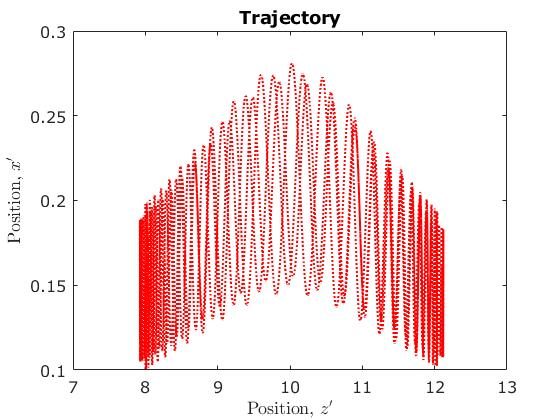
\includegraphics[scale=0.4]{problem4a/trajectory_zx_5000.jpg}
}
\caption{The trajectory in the $(z, x)$ plane with AB3 scheme and $N=5000$ timesteps, and final time $T' = 5\pi$.}
\label{problem 1.1}
\end{figure}

\item
Plot the 3D trajectory of the particle of the same simulation over plotted region.

The trajectory is shown in Figure \ref{problem 1.2}.
\begin{figure}[h]
\centering
\vbox{
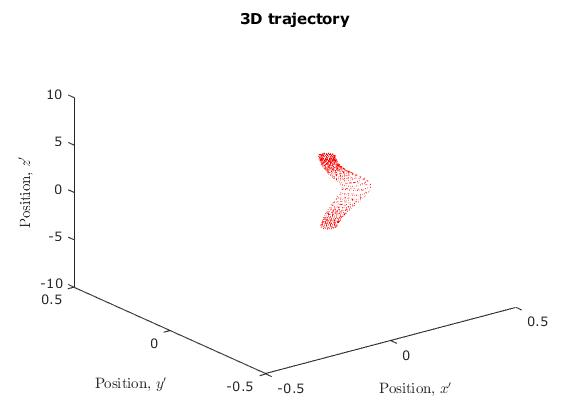
\includegraphics[scale=0.4]{problem4a/trajectory_3d_5000.jpg}
}
\caption{The trajectory in the $(x, y, z)$ plane with AB3 scheme and $N=5000$ timesteps, and final time $T' = 5\pi$.}
\label{problem 1.2}
\end{figure}

\item Plot the evolution of normalized magnetic moment.

The plot is shown in Figure \ref{problem 1.3}, where we observe that with the increase of timesteps $N$, the conservation gets better.

\begin{figure}[h]
\centering
\vbox{
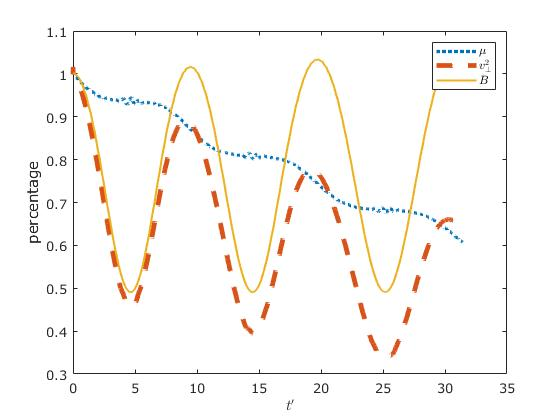
\includegraphics[scale=0.29]{problem4a/magnetic_5000.jpg}
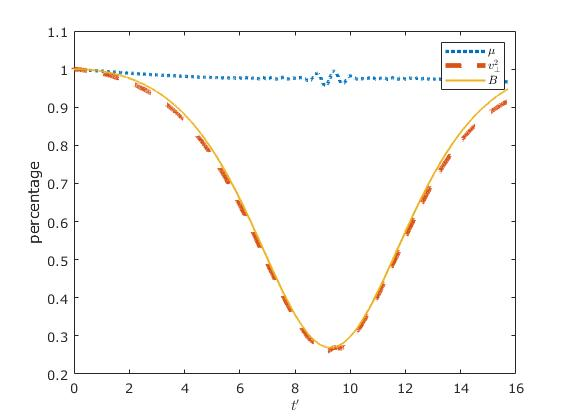
\includegraphics[scale=0.29]{problem4a/magnetic_10000.jpg}
}
\vbox{
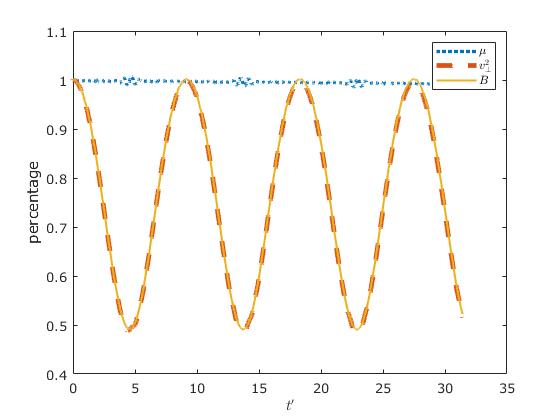
\includegraphics[scale=0.29]{problem4a/magnetic_20000.jpg}
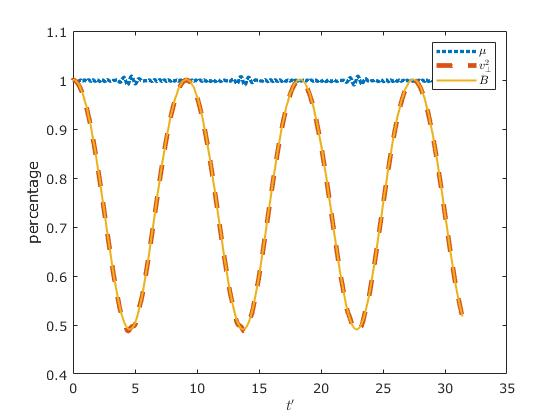
\includegraphics[scale=0.29]{problem4a/magnetic_50000.jpg}
}
\caption{The normalized magnetic moment $\mu$, normalized perpendicular velocity $v_\perp^2 $ and magnetic field magnitude $B$. Top: number of time steps $N = 5000, 10000$. Bottom: $N = 20000, 50000$.}
\label{problem 1.3}
\end{figure}

\item
Plot the evolution of normalized kinetic energy.

The plot is shown in Figure \ref{problem 1.4}, where we observe that with the increase of timesteps $N$, the conservation gets better.

\begin{figure}[h]
\centering
\vbox{
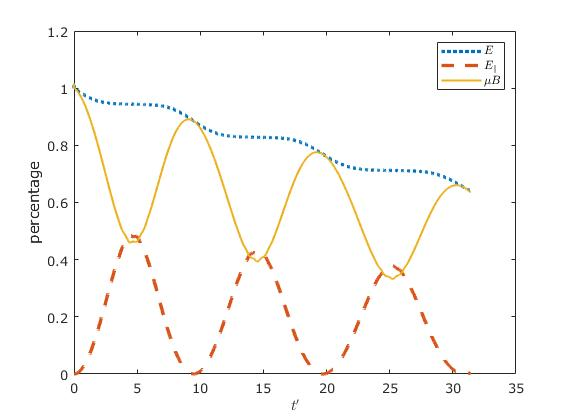
\includegraphics[scale=0.29]{problem4a/energy_5000.jpg}
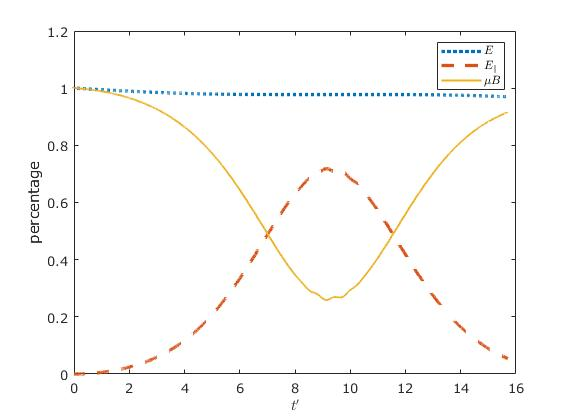
\includegraphics[scale=0.29]{problem4a/energy_10000.jpg}
}
\vbox{
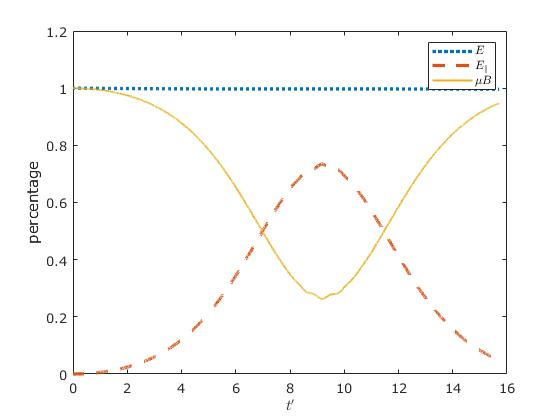
\includegraphics[scale=0.29]{problem4a/energy_20000.jpg}
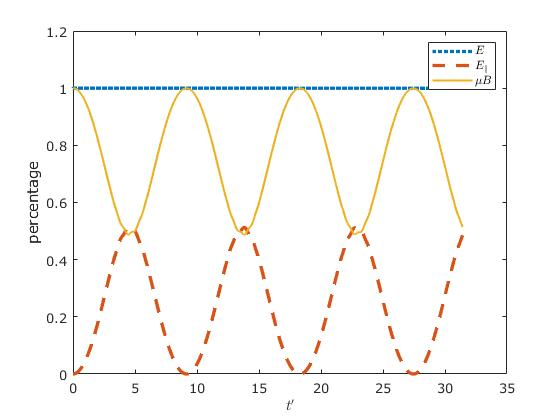
\includegraphics[scale=0.29]{problem4a/energy_50000.jpg}
}
\caption{The normalized total kinetic energy $E$, normalized parallel kinetic energy $E_\parallel $ and $\mu B$. Top: number of time steps $N = 5000, 10000$. Bottom: $N = 20000, 50000$.}
\label{problem 1.4}
\end{figure}

\end{enumerate}

\item
Implementation of Adaptive Runge-Kutta (RK45).

\begin{enumerate}
\item
Run AB3 with $N=10000$ steps and compute the error at $\Omega t = 20\pi$. Set relative tolerance for RK45 to the same value, determine how many time steps it requires.

For AB3, $e = 5.3978\times 10^{-6} $. For RK45, the number of time steps with $RelTol = e$ is $N = 993$.

\item
Plot the trajectory for RK45 with $RelTol = 4\times 10^{-3} $. How many steps does this require? Total relative error?

The plot is shown in Figure \ref{problem 2.2}, where the number of time steps is $N = 257$, and relative total error with repect to analytical solution $e = 4.94\times 10^{-3} $.

\begin{figure}[h]
\centering
\vbox{
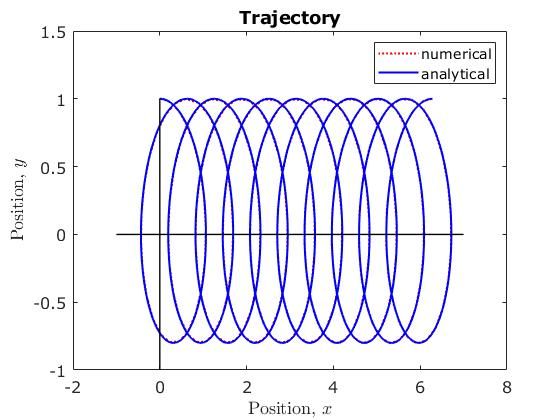
\includegraphics[scale=0.4]{problem4b/trajectory.jpg}
}
\caption{The trajectory in the $(x, y)$ plane with RK45 scheme and $N=257$ timesteps, and final time $T' = 20\pi$.}
\label{problem 2.2}
\end{figure}

\item
How many RK45 steps required if change $RelTol = 1\times 10^{-6} $. Total relative error? Why total error larger than specified tolerance?

$N = 1153$ for $RelTol = 1\times 10^{-6} $. The relative total error is $e = 1.266\times 10^{-6} $.

It's larger than $RelTol$ since in \texttt{ode45}, the program uses the solution of $5^{th} $ order method to estimate the real solution for adaptive control of the step size of the $4^{th} $ order method. However, the solution of $5^{th} $ order method is not accurate so it still has some small error, which makes the final relative error slightly larger than $RelTol$.

\end{enumerate}

\item Magnetic Mirror Integration with RK45.
\begin{enumerate}
\item
Using conservation of energy as a measure of accuracy, how many AB3 steps need for energy loss less than $0.1\%$? Set RK45 $RelTol = 10^{-3} $, how mant steps require, error in energy?

For AB3, $N = 2208$. 

For RK45, $N = 341$, error in energy is $3.24\times 10^{-3} $.

\end{enumerate}


\end{enumerate}


\end{document}